\documentclass{beamer}
\usetheme[numbering=progressbar]{focus}
\usepackage{tikz}
\usepackage{listings}
\usetikzlibrary{positioning}
\usetikzlibrary{shapes,arrows}
\usepackage{transparent}
\usepackage{fancyvrb}
\usepackage{listings}
\definecolor{main}{RGB}{47, 161, 219}
%\definecolor{textcolor}{RGB}{128, 128, 128}
\definecolor{background}{RGB}{240, 247, 255}
\definecolor{textcolor}{RGB}{85, 87, 83}
\title{Cryptography Workarounds For Law Enforcement}
\subtitle{Snake oil Crypto, D4 and other tricks}
\author{Jean-Louis Huynen}
\titlegraphic{
\includegraphics[scale=.5]{logo-circl.pdf}}
\institute{Team CIRCL \\ }
\date{2019/11/27}

\begin{document}

\begin{frame}
    \maketitle
\end{frame}

\begin{frame}
        \frametitle{Outline}

        \begin{itemize}
          \item Cryptography 101,
          \item Brute Force 101,
          \item Encryption an Law Enforcement,
          \item Pretty Good Privacy / GnuPG
          \item Use-Case: RSA,
          \item First Hands-on: Understanding RSA,
          \item Snake-Oil-Crypto: a primer,
          \item Second Hands-on: RSA in Snake-Oil-Crypto,
          \item D4 passiveSSL Collection,
          \item Interactions with MISP.
        \end{itemize}

\end{frame}

\begin{frame}
  \begin{center}
    {\bf Cryptography 101}
  \end{center}
\end{frame}


\begin{frame}
  \frametitle{Cryptography Concepts}
        \begin{itemize}
          \item {\bf Plaintext} P: Text in clear,
          \item {\bf Encryption} E: Process of disguising the plaintext to hide its content,
          \item {\bf Ciphertext} C: Result of the Encryption process,
          \item {\bf Decryption} D: Process of reverting encryption, transforming C
            into P,
          \item {\bf Encryption Key} EK: Key to encrypt P into C,
          \item {\bf Decryption Key} DK: Key to decrypt C into P,
          \item {\bf Cryptanalysis}: Analysis of C to recover P without knowing K.
        \end{itemize}

\end{frame}

\begin{frame}
        \frametitle{Cryptography Services}

        \begin{itemize}
          \item {\bf Confidentiality }: Ensure the secrecy of the message except for
            the {\bf intended } recipient,
          \item {\bf Authentication }: Proving a party's identity,
          \item {\bf Integrity }: Verifying that data transmitted were not altered,
          \item {\bf Non-repudiation }: Proving that the sender sent a given message.
        \end{itemize}

\end{frame}

\begin{frame}
        \frametitle{Type of Encryption Applications}

        \begin{itemize}
          \item {\bf In-transit encryption}: protects data while it is
            transferred from one machine to another,
          \item {\bf At-rest encryption}: protects data stored on one machine.
          %\item {\bf Perfect Forward Secrecy}
        \end{itemize}

\end{frame}

\begin{frame}
        \frametitle{Encryption most important concepts}

        \begin{itemize}

          \item {\bf Confusion}: Obscures the relationship between the Cipher
            Text and the key. In a perfect cipher, changing one bit of the key
            should change all bits of the Cipher Text.

          \item {\bf Diffusion}: Hides relationship between the Plain Text and the
            Cipher Text (eg. symbols frequencies). In a perfect cipher changing
            a single bit of the Plain Text bit affects at least half of the Cipher Text bits.

          \item {\bf Kerckhoffs's Principle}: The algorithm can be public:

        \begin{quote}
          It [cipher] should not require secrecy, and it should not be a problem if it falls into enemy hands.
        \end{quote}

        \end{itemize}


        \vspace{5 mm}
\center
        {  \bf There is no security in obscurity.}

\end{frame}


\begin{frame}[allowframebreaks]
        \frametitle{Attackers model}
        {\bf Black Box} - Attackers may only see inputs / outputs:
        \begin{itemize}
          \item {\bf Ciphertext-Only Attackers (COA) :} see only the ciphertext,
          \item {\bf Known-Plaintext Attackers (KPA):} see ciphertext and plaintext,
          \item {\bf Chosen-Plaintext Attacker (CPA):} encrypt plaintext, and
            see ciphertext, 
          \item {\bf Chosen-Ciphertext Attakers (CCA):} encrypt plaintext,
            decrypt ciphertext.
        \end{itemize}

        \framebreak

        {\bf Grey Box} - Attackers see cipher's implementation:
        \begin{itemize}
          \item {\bf Side-Channel Attacks:} study the behavior of the
            implementation, eg. {\bf timing attacks }\footnote{\url{https://cryptojedi.org/peter/data/croatia-20160610.pdf}}:
            \begin{itemize}

              \item Osvik, Shamir, Tromer~\cite{aes2006}: Recover AES-256 secret
                key of Linux’s dmcrypt in just 65 ms
              \item AlFardan, Paterson~\cite{lucky13}: “Lucky13” recovers plaintext of CBC-mode encryption in pretty much all TLS implementations
              \item Yarom, Falkner~\cite{gpg2014}: Attack against RSA-2048 in GnuPG 1.4.13: “On average, the attack is able to recover 96.7\% of the bits of the secret key by observing a single signature or decryption round.”
              \item Benger, van de Pol, Smart, Yarom~\cite{openssl2014}: “reasonable level of success in recovering the secret key” for OpenSSL ECDSA using secp256k1 “with as little as 200 signatures”

            \end{itemize}

        \framebreak
        Most recent timing attack: {\bf TPM-fail }~\cite{244048}

        \vspace{10 mm}

            \begin{figure}[h!]
              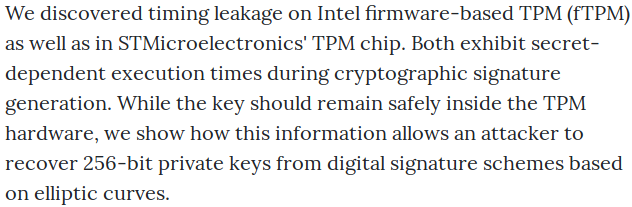
\includegraphics[width=250px]{./tpmfail.png}
            \end{figure}

        \framebreak

          \item {\bf Invasive Attacks:} 

            \begin{itemize}
              \item injecting faults~\cite{Matsuda2018},

                \vspace{10 mm}

                \begin{figure}[h!]
                  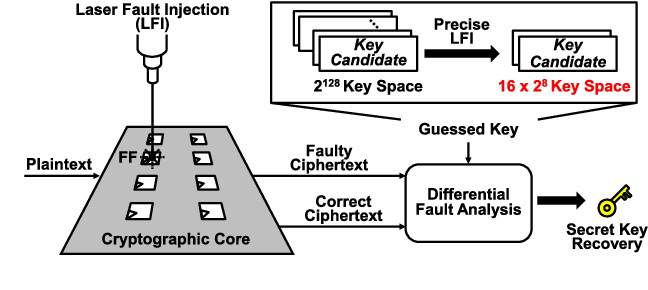
\includegraphics[width=250px]{./faultInjection.png}
                \end{figure}

        \framebreak

              \item decapping chips~\footnote{~\url{https://siliconpr0n.org/wiki/doku.php?id=decap:start}}, reverse engineering~\footnote{~\url{http://siliconzoo.org}}~\footnote{~\url{http://degate.org}}, etc~\cite{heckm2018}.

           \end{itemize}
 
        \end{itemize}

                \begin{figure}[h!]
                  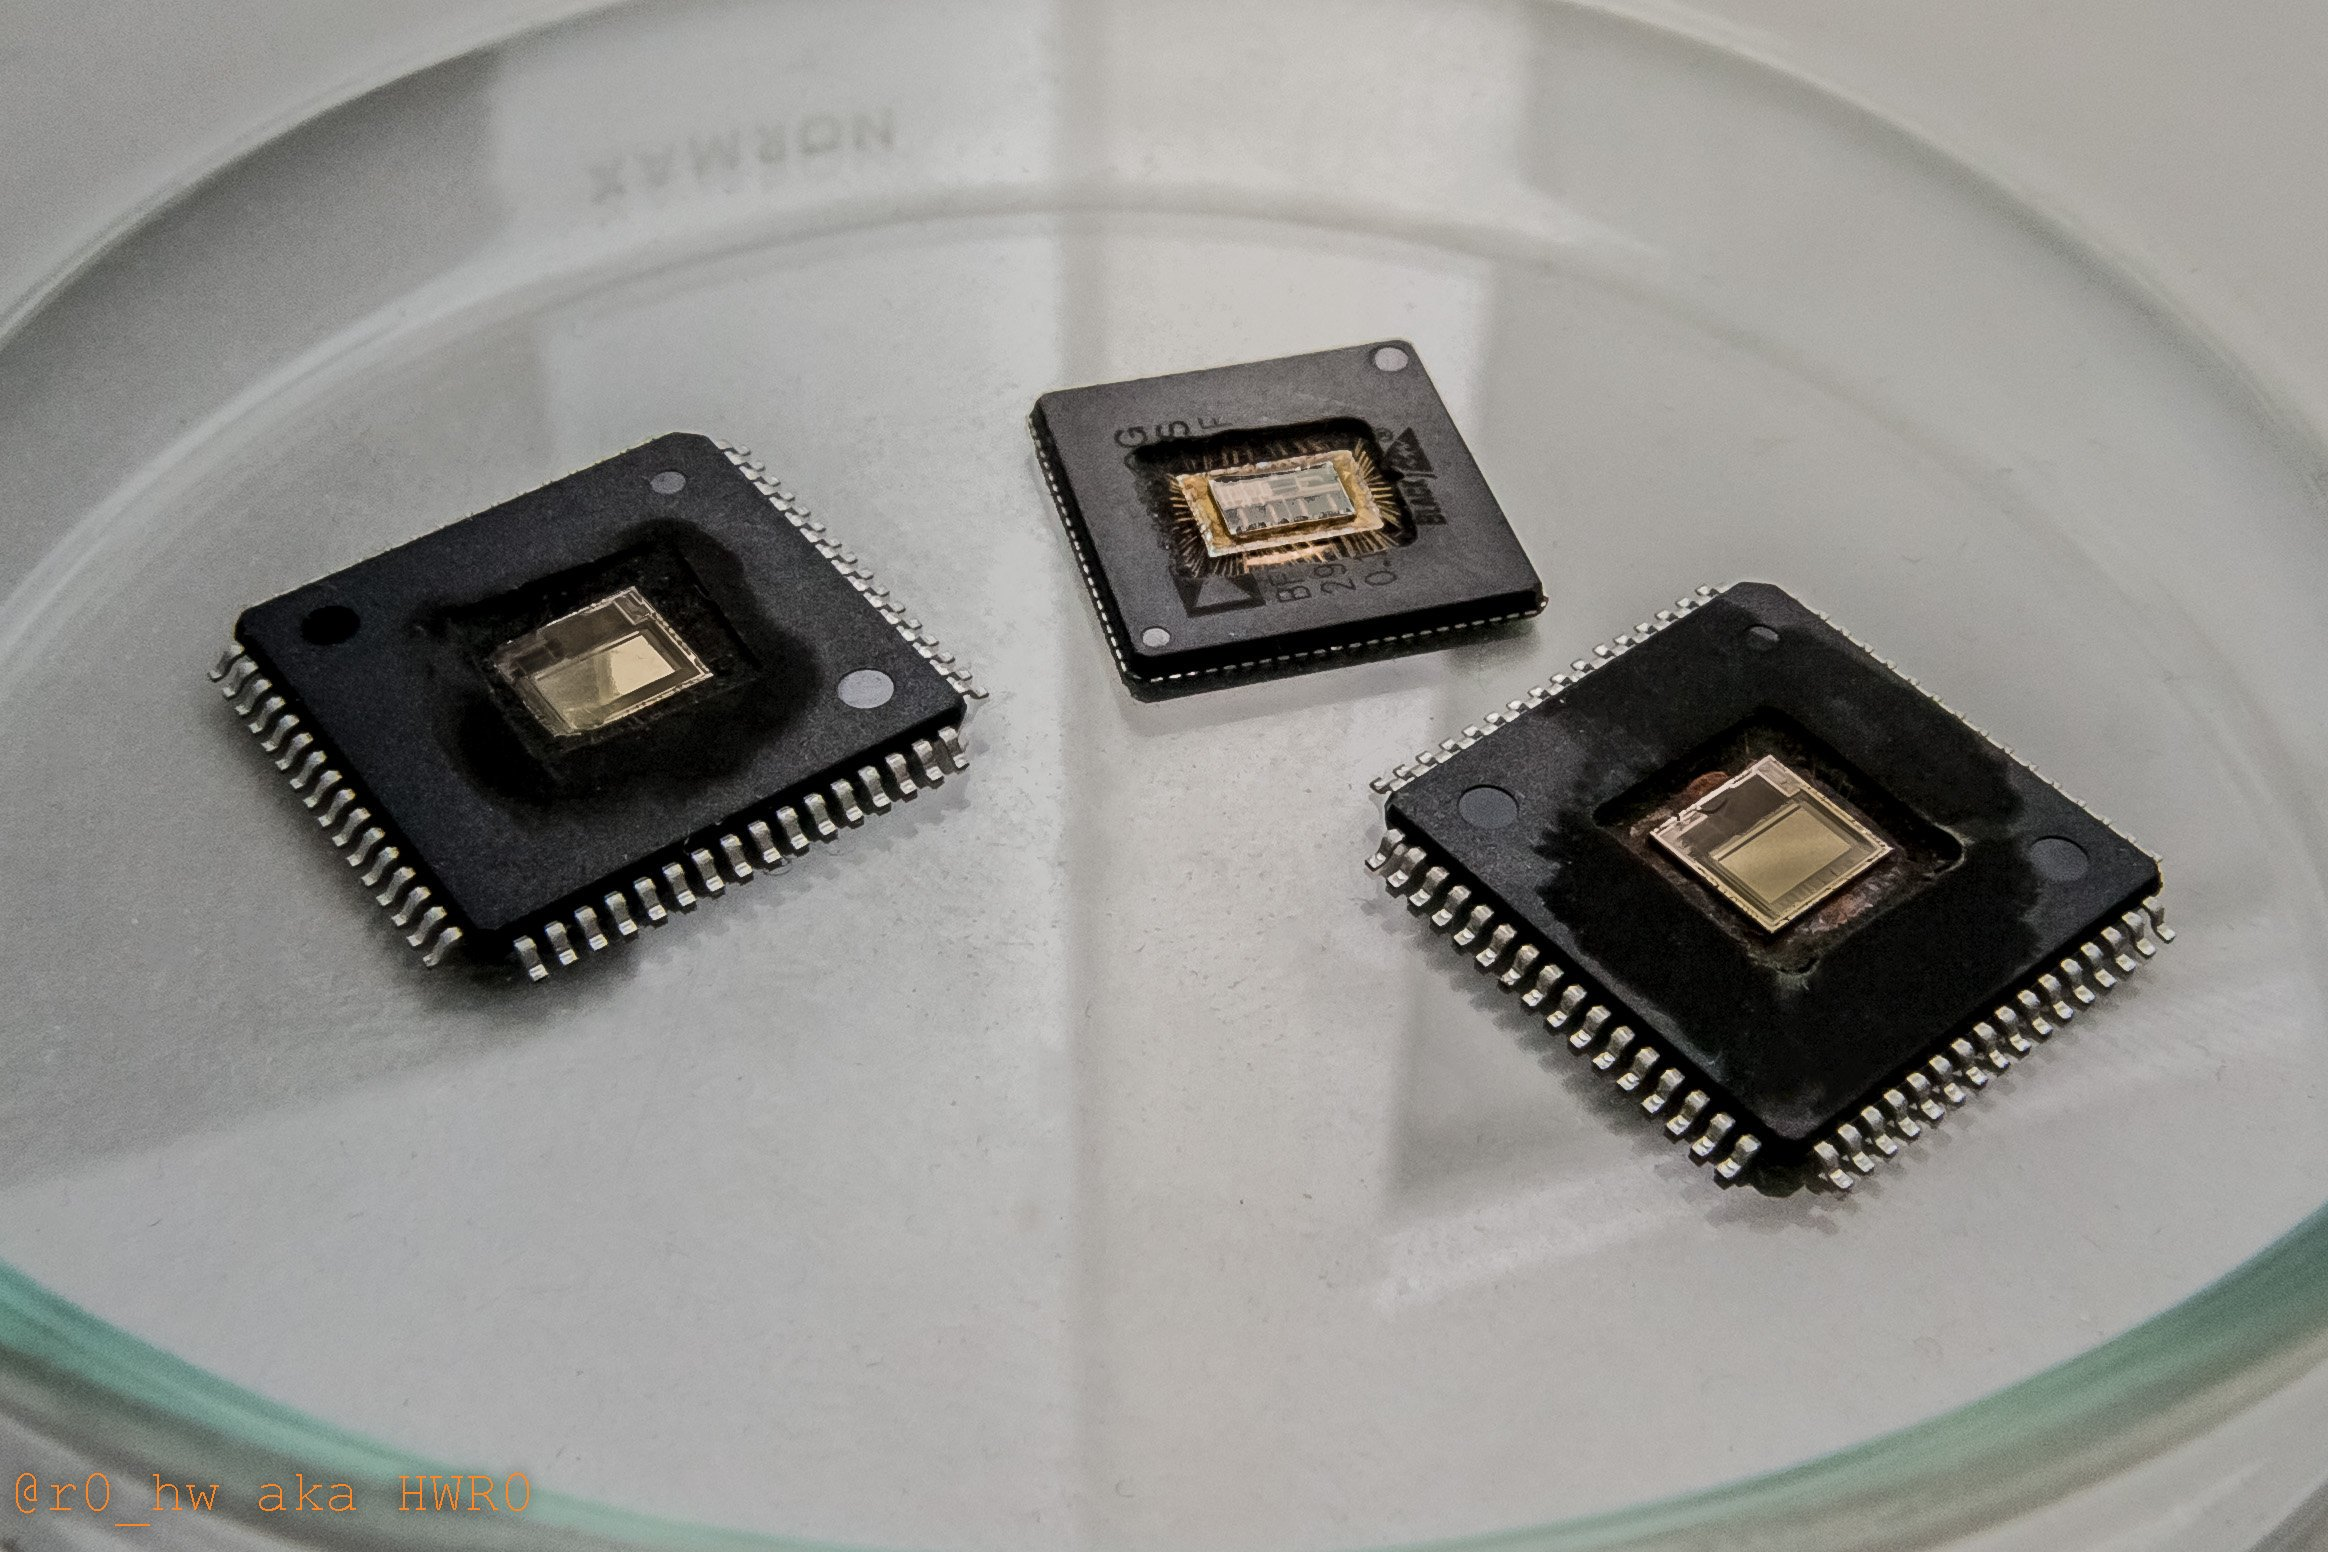
\includegraphics[width=.49\textwidth]{./decaping.jpg}%
                  \hfill
                  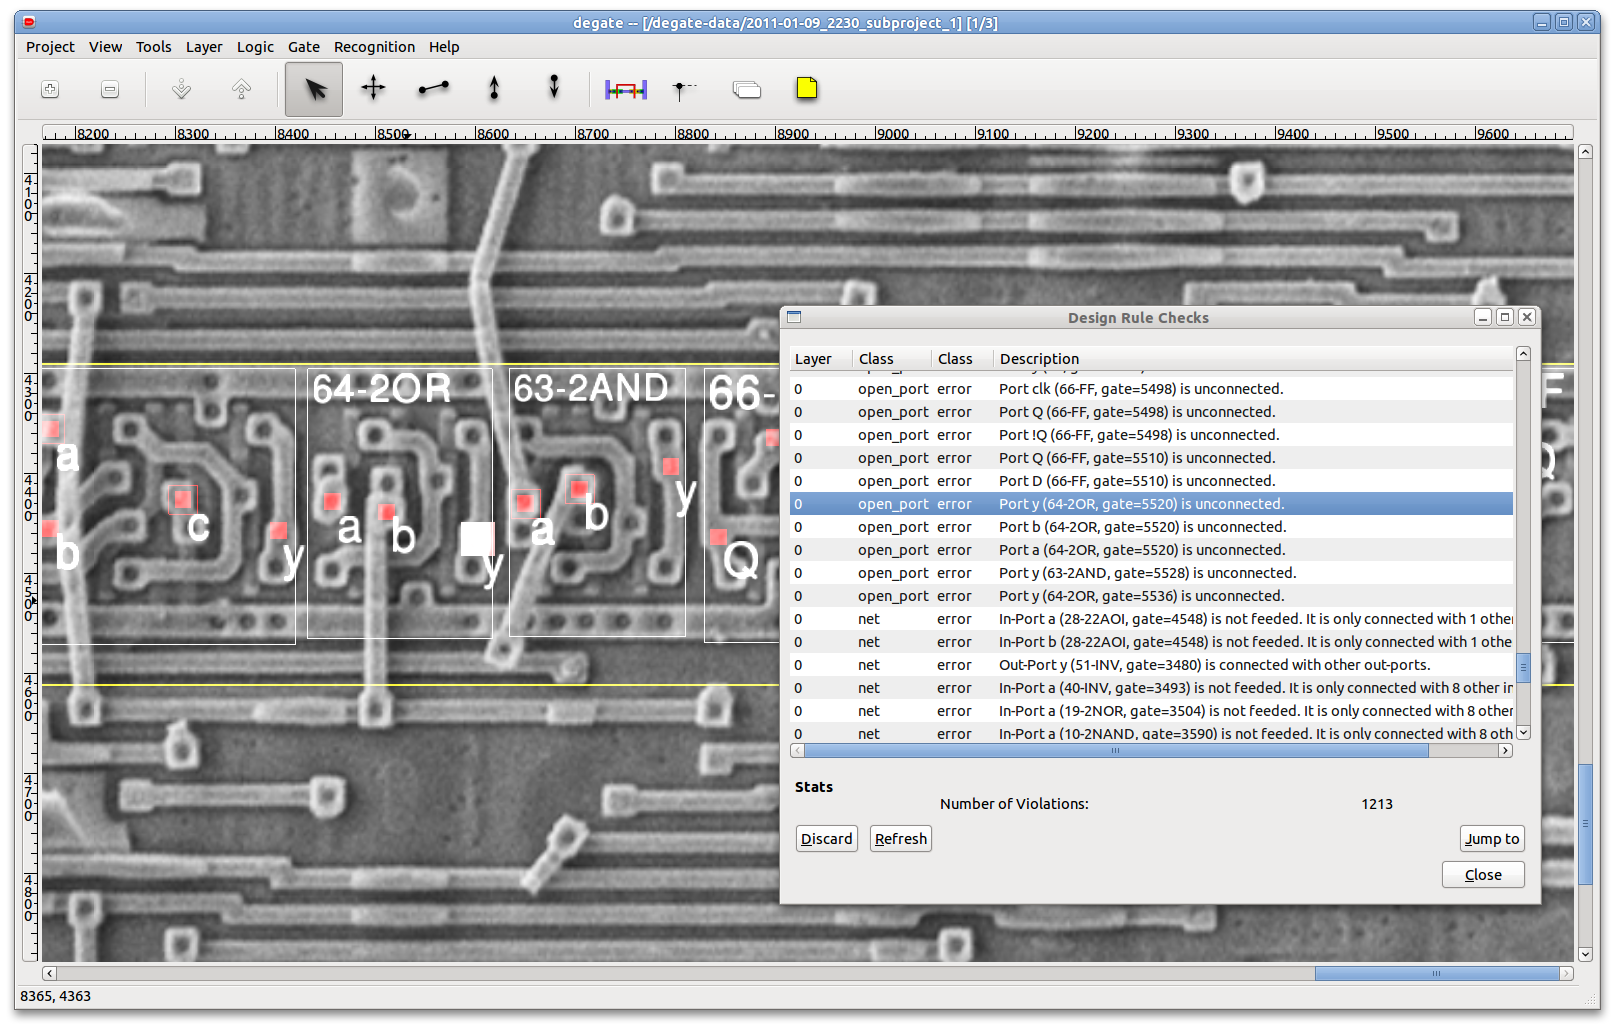
\includegraphics[width=.49\textwidth]{./degate.png}
                \end{figure}

\end{frame}

\begin{frame}
        \frametitle{Security Notions}

        \begin{itemize}
          \item {\bf Indistinguishability (IND) :} Ciphertexts should be
            indistinguishable from random strings,

          \item {\bf Non-Malleability (MD):} ``Given a ciphertext $C_1 = E(K, P 1)$,
it should be impossible to create another ciphertext, $C_2$ , whose corresponding
plaintext, $P_2$ , is related to $P_1$ in a meaningful way.''

        \end{itemize}

        \vspace{1 mm}

        Semantic Security (IND-CPA) is the most important security feature:
        \begin{itemize}
          \item Ciphertexts should be different when encryption is performed
            twice on the same plaintext,
          \item To achieve this, randomness is introduced into encryption /
            decryption: 

        \begin{itemize}
          \item $C = E(P, K, R)$
          \item $P = D(C, K, R)$
        \end{itemize}

        \end{itemize}
       \end{frame}


\begin{frame}
        \frametitle{Semantic Security}
        \begin{figure}
          \centering
          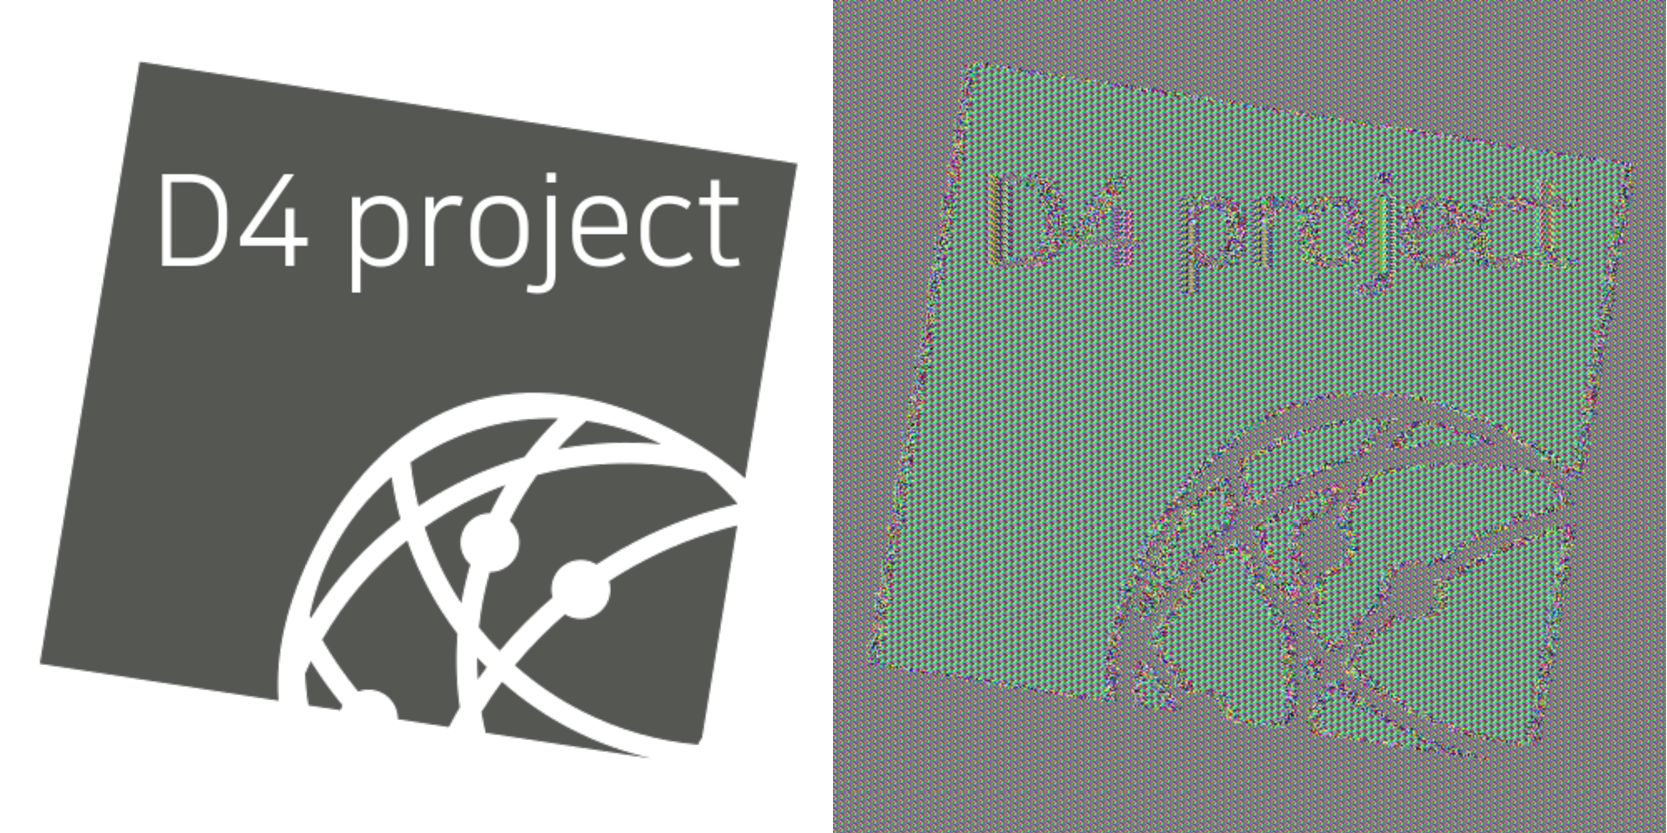
\includegraphics[width=\textwidth]{d4-ecb.pdf}
          \caption{Image encrypted with AES-ECB}
        \end{figure}
        
\end{frame}


\begin{frame}
        \frametitle{Semantic Security}

        IND-CPA should not leak information about the PlainText as long as the
        key is secret:

        \begin{itemize}
          \item $C^1 = E(K, P^1)$, $C^2 = E(K, P^2)$, what are the couples?
          \item the same message encrypted twice should return two different CipherText,
          \item one way to achieve this is to introduce randomness in the
            encryption process: $C = E(K ,R ,P )$ where R is fresh random bits,
          \item C should not be distinguishable from random bits.
        \end{itemize}

        {\bf No Semantic Security without randomness}

\end{frame}

\begin{frame}
        \frametitle{Randomness}

        \begin{itemize}
          \item {\bf Entropy}: (measure of) disorder in a system,
          \item {\bf Random Number Generator}: a source of entropy, or uncertainty,
          \item {\bf Pseudo Random Number Generator}: a crypto algorithm that
            produces a stream of random (hopefully) bits from the RNG.
          \item there are cryptographic and non-cryptographic (predictable) PRNG,
          \item there are software-based, and hardware-based PRNG.
        \end{itemize}

            \begin{figure}[h!]
              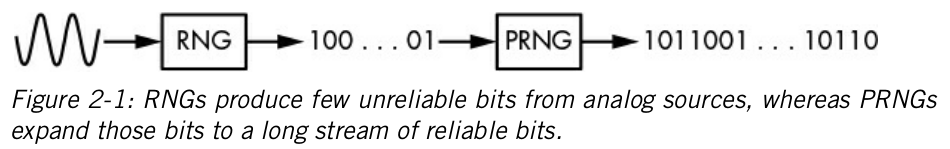
\includegraphics[width=250px]{./random.png}
            \end{figure}

         {\bf Bad entropy sources are a disaster for crypto-systems (ask casinos).}

\end{frame}

\begin{frame}
        \frametitle{Quantifying Security}
       RSA 2048 is roughly 100 bits security. 
        \begin{itemize}
          \item The key size is different for the ``bits of security'',
          \item ``n-bits'' of security means that $2^n$ operations are needed to
            compromise break a cipher. 
        \end{itemize}

\end{frame}


\begin{frame}
        \frametitle{Type of encryption}

        \begin{itemize}
          \item Symmetric encryption: two parties share a key to encrypt and decrypt,
          \item Asymmetric encryption, there are two keys:
            
        \begin{itemize}
        \item one can encrypt -- this one is public -- so public can send you
          encrypted messages,
         \item another one can decrypt -- this one is private -- so you can
           decrypt the message encrypted for you.
        \end{itemize}
        \item Obviously, one can not compute the private key from the public key.
        \item as the public key is public, the attacker model of public-key
          cryptography is Chosen Plaintext Attacker.
        \end{itemize}

\end{frame}

\begin{frame}
  \begin{center}
    {\bf Brute Force 101}
  \end{center}
\end{frame}


\begin{frame}
        \frametitle{Brute Forcing - Basics}
        2 Approaches:
        
        \begin{itemize}
          \item {\bf Exhaustive Key Search:}
        \begin{itemize}
          \item n bits key : $2^n$ trials,
          \item most likely around half of the trials ($2^{n-1}$),
          \item no memory needed.
        \end{itemize}
          \item {\bf Code Book Attack}
        \begin{itemize}
        \item Pre-Compute $C = E(P, K)$ for all keys $K$,
        \item store $2^{k}$ keys,
        \item for a given $C$, look up for $K$.
        \end{itemize}
        \end{itemize}

\end{frame}

\begin{frame}
        \frametitle{Brute Forcing - Key Search}
        Key search is testing each possible keys by trial and errors:
        \begin{itemize}
          \item We usually consider that one trial requires 1 ns to complete,
        \begin{itemize}
          \item n bits key : $2^n$ trials,
          \item 128 bits of security : $2^{128}$ trials,
          \item $2^{88}$ ns = age of the universe,
          \item with ns by trial, we need $2^{40}$ times the age of the universe
            to cover all keys,
        \end{itemize}
          \item some attacks can be done in parallel (sequentially independent operations): 
        \begin{itemize}
          \item For one million cores:
          \item length of one million in bits is $log2(1000000) = 19,93$
          \item $2^{128}/2^{20} = 2{108}$
          \item $2^{20}$ times the age of the universe.
        \end{itemize}
        \end{itemize}
\end{frame}


\begin{frame}[allowframebreaks]
        \frametitle{Brute Forcing - TMTO}
\begin{quote}
  ``It usually takes a long time to find a shorter way.''
\end{quote}
        {\bf T}ime-{\bf M}emory {\bf T}rade {\bf O}ff:
        \begin{itemize}
         \item Chosen Plaintext Attack,
         \item Hellman in 1980,
         \item It is a trade-off between Exhaustive Key Search, and Code Book Attacks,
         \item more expensive than an exhaustive search as it requires:
        \begin{itemize}
        \item $2^{n}$ one-time pre-computations, using one known plaintext,
        \item the storage of these $2^{n}$ results,
        \item the results are chains, that also have a cost to invert.
        \end{itemize}
         \item speed-up attacks against memory space,
         \item useful when routinely attacking a cipher (eg. computing 1.68 To of tables allows for almost instant cracking of A5/1 cipher used in GSM communications).
        \end{itemize}
        
            \begin{figure}[h!]
              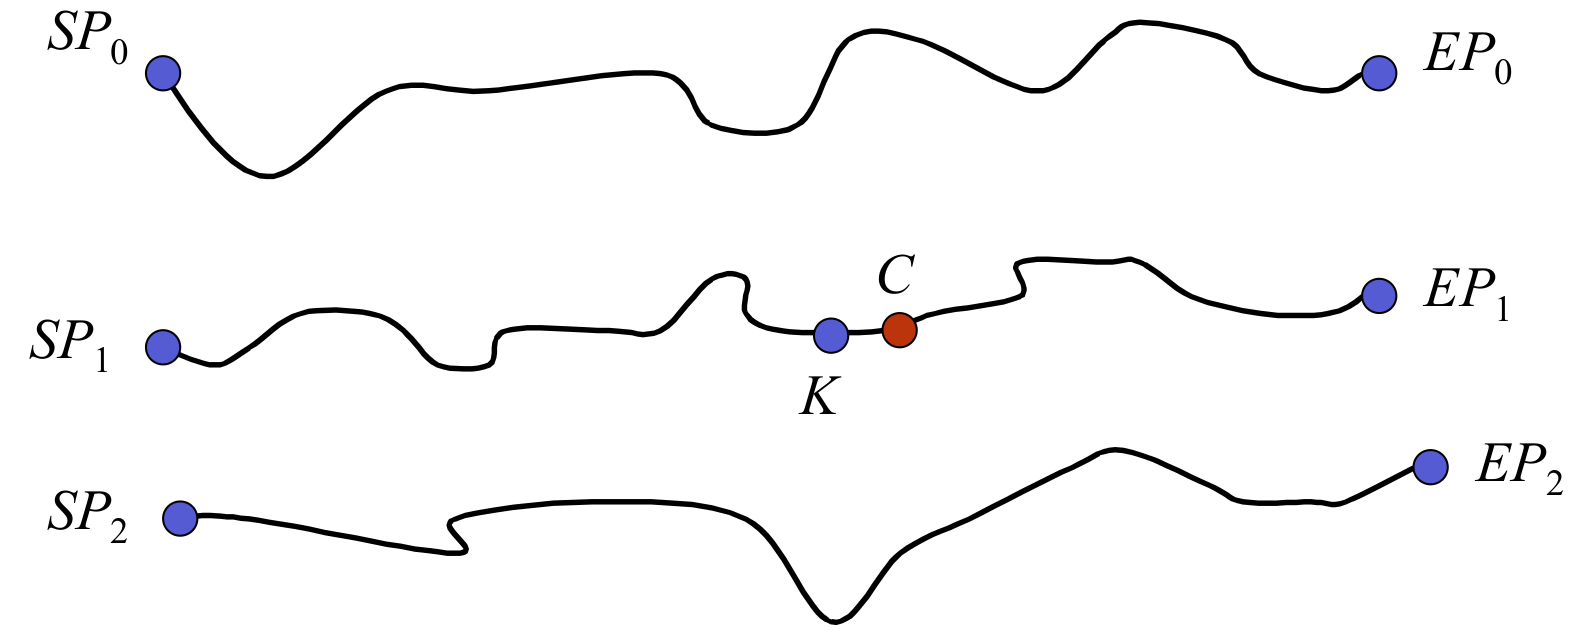
\includegraphics[width=220px]{./chains1.png}
            \end{figure}


            \begin{figure}[h!]
              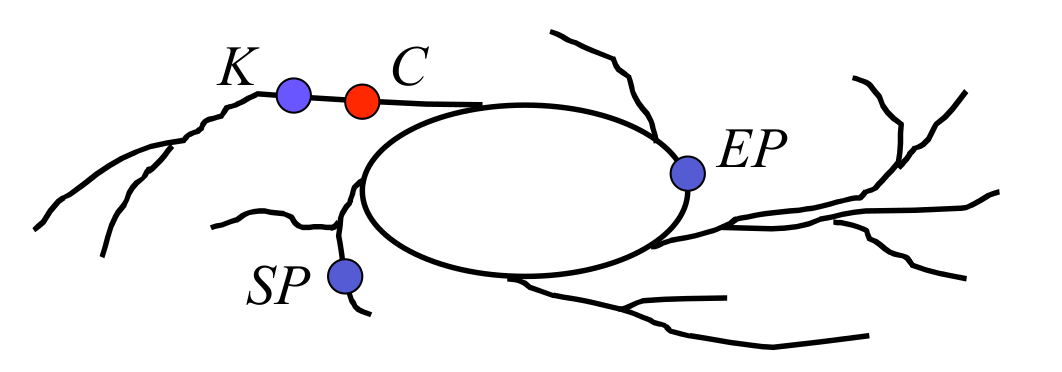
\includegraphics[width=220px]{./chains2.png}
            \end{figure}

        {\bf Rainbow Tables are an improved version of Hellman's algorithm.}
\end{frame}

\begin{frame}
        \frametitle{How Keys are generated anyway?}
        There are three ways keys can be generated:
        \begin{itemize}
          \item By {\bf Randomly} choosing the key from a PRNG,
          \item by {\bf Deriving} the key from a password using a Key Derivation Function,
          \item by using a {\bf Key agreement protocol} that requires
            interactions between involved parties.
        \end{itemize}
\end{frame}

\begin{frame}
  \begin{center}
    {\bf Encryption and Law Enforcement}
  \end{center}
\end{frame}

\begin{frame}
        \frametitle{2016 ENISA / EUROPOL joint statement}
        \begin{itemize}
          \item In the arms race between cryptographers and crypto-analysts. In
            terms of practical breaks, cryptographers are miles ahead.
          \item In a society that is ever more depending on the correct
            functioning of electronic communication services, technical
            protection of these service is mandatory,
          \item In the face of serious crimes, law enforcement may lawfully
            intrude privacy or break into security mechanisms of electronic communication,
          \item {\bf proportionality} - collateral damages (class breaks)
          \item Resolving the encryption dilemma: collect and share best
            practices to circumvent encryption.
        \end{itemize}
\end{frame}

\begin{frame}[allowframebreaks]
        \frametitle{Encryption Workarounds~\cite{kerr2017}}
        \begin{quote}
          Any effort to reveal an unencrypted version of a target's data that
          has been concealed by encryption.
        \end{quote}
        \begin{itemize}
          \item {\bf Try to get the key:}
          \begin{itemize}
        \item {\bf Find the key:} 
          \begin{itemize}
          \item physical searches for keys,
          \item password managers,
          \item web browser password database,
          \item in-memory copy of the key in computer's HDD / RAM.
          \item seize the key (keylogger).
          \end{itemize}
        \item {\bf Guess the key:},
          \begin{itemize}
            \item Whereas encryption keys are usually too hard to guess (eg.
              128bits security is $2^{128}$ trials (universe is $2^{88}$ ns old)),
            \item passphrases are usually shorter to be memorizable, and are
              linked to the key,
            \item some systems have limitations on sorts of passwords (eg. 4/6
              digits banking application),
            \item educated guess on the password from context,
            \item educated guess from owner's other passwords,
            \item dictionaries and password generation rules (\footnote{\url{https://hashcat.net/hashcat/}}).
            \item Offline / online attacks (eg. 13 digits pw: 25.000 on an
              iphone VS matter of minutes offline),
            \item + beware devices protection when online (eg. iphone erase on repeated failures).
          \end{itemize}
         
        \item {\bf Compel the key:}
          \begin{figure}
            \centering
            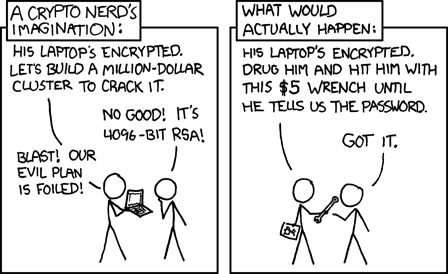
\includegraphics[width=180px]{security.png}
          \end{figure}
        \end{itemize}

          \item {\bf Try to access the PlainText without the key:}

        \begin{itemize}
          \item {\bf Exploit a Flaw:}

            \begin{itemize}
              \item Weakness in the algorithm (more on that later),
              \item weakness in the random-number generator (more on that later),
              \item weakness in the implementation,
              \item bugs (eg. Gordon's exploit on android in
                2015\footnote{\url{https://cve.circl.lu/cve/CVE-2015-3860}}),
              \item backdoors (eg. NSA NOBUS -Bullrun program- Dual EC-DRBG~\cite{eprint-2015-26238}
            \end{itemize}

          \item {\bf Access PlainText when in use:}

            \begin{itemize}
              \item Access live system memory,
              \item especially useful against Full Disk Encryption,
              \item Seize device while in use,
              \item remotely hack the device,
              \item ``Network Investigative Technique'' (eg. Playpen case
                against tor).
            \end{itemize}

\pagebreak 

          \item {\bf Locate a PlainText copy:}

            \begin{itemize}
              \item Avoid encryption entirely,
              \item cloud providers (eg. emails),
              \item remote cloud storage (eg. iCloud),
            \end{itemize}
 
        \end{itemize}

       \end{itemize}

      \vspace{5mm}

       {\bf Takeaways:}
       \begin{itemize}
        \item {\bf No workaround works every time:}  the fact that a target used
          encryption does not mean that the investigation is over.
        \item {\bf some workarounds are expensive:} exploiting.
        \item {\bf expertise may be have to be found outside of the
            governments:} vendors' assistance?
       \end{itemize}

 
        \framebreak

      Technically, we can retain that crypto-systems have weaknesses:

      \begin{itemize}
        \item key generation,
        \item key length,
        \item key distribution,
        \item key storage,
        \item how users enter keys into the crypto-system,
        \item weakness in the algorithm itself / implementation,
        \item system / computer running the algorithm,
        \item crypto system used in different points in time,
        \item {\bf users.}
      \end{itemize}

       
\end{frame}

\begin{frame}
        \frametitle{When cryptography helps investigations}
        \begin{itemize}
         \item authentication mechanisms between peers,
         \item openGPG can leak a lot of metadata
        \begin{itemize}
          \item key ids,
          \item subject of email in thunderbird,
        \end{itemize}
          \item Bitcoin's Blockchain is public,
          \item correlating these data with external sources can yields
            interesting insights,
          \item More on this in AIL workshop.
        \end{itemize}

\end{frame}

\begin{frame}
  \begin{center}
    {\bf Pretty Good Privacy / Gnu Privacy Guard}
  \end{center}
\end{frame}

\begin{frame}
  \frametitle{Pretty Good Privacy / Gnu Privacy Guard}
  \begin{itemize}
    \item PGP was Invented By Phil Zimmermann in 1991,
    \item Hybrid Cipher: asymmetric encryption with symmetric encryption,
    \item allows to sign communications and files for authentication,
    \item very low vulnerability count over the years~\footnote{https://cve.circl.lu/search/gnupg/gnupg},
    \item One can generate collisions on short IDs though\footnote{\url{https://github.com/lachesis/scallion/}},
    \item no Perfect Forward Secrecy,
    \item but sessions keys.
  \end{itemize}
\end{frame}

\begin{frame}
  \frametitle{Pretty Good Privacy / Gnu Privacy Guard}
            \begin{figure}[h!]
              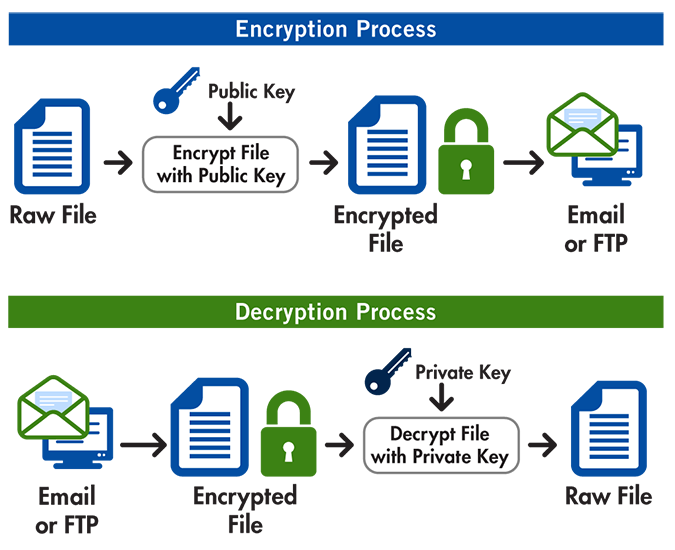
\includegraphics[width=250pt]{./gpg.png}
            \end{figure}
\end{frame}

\begin{frame}
  \frametitle{Pretty Good Privacy / Gnu Privacy Guard}
            \begin{figure}[h!]
              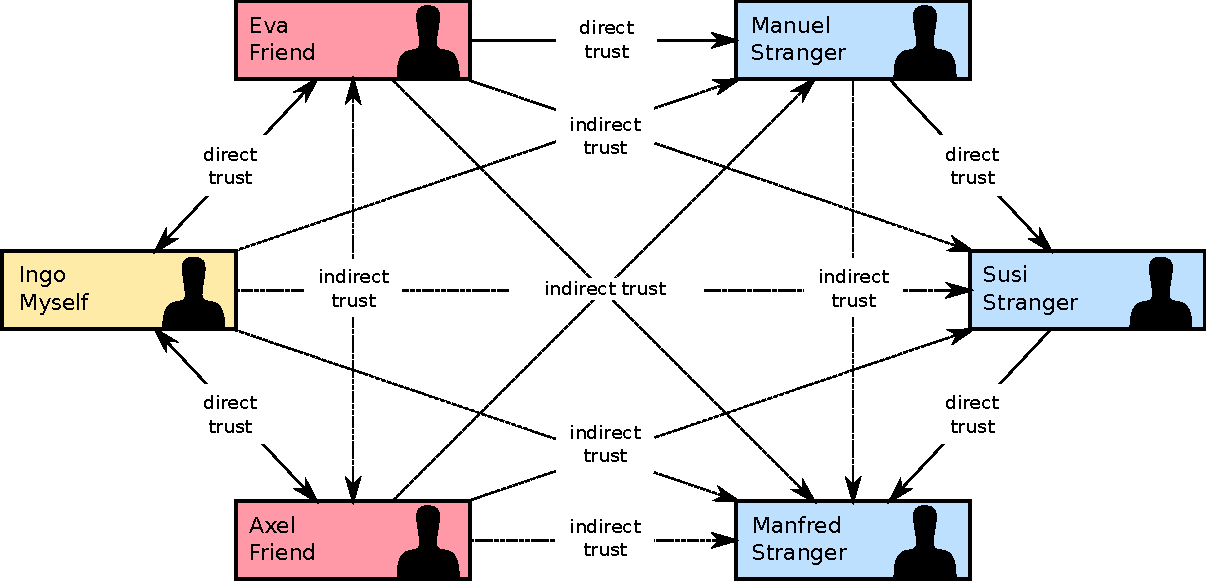
\includegraphics[width=300pt]{./wot.pdf}
            \end{figure}
\end{frame}

\begin{frame}[fragile]
  \frametitle{Gnu Privacy Guard: Session keys}

  \begin{itemize}
    \item {\bf Hands-on}
  \begin{lstlisting}
  Move into ~/hands-on/GPGsessions
  \end{lstlisting}
    \item We create two keys, one for the person being the focused of an
      investigation A (The Very Bad Guy), and one for a witness B (Mr. Good Guy),
    \item then, we encrypt two messages:
      \begin{itemize}
       \item one from A to B: to\_encrypt\_relevant.asc,
       \item and a note, form B to B (note): to\_encrypt\_irrelevant.asc, 
      \end{itemize}
    \item B's passphrase is ``goodguypassphrase'',
    \item act as B and extract the session key for to\_encrypt\_relevant.asc,
    \item act as a cop and use the session key to decrypt
      to\_encrpyt\_relevant.asc,
    \item verifies that it does not work to decrypt to\_encrypt\_irrelevant.asc.
  \end{itemize}
\end{frame}



\begin{frame}
  \begin{center}
    {\bf Broken Implementations}
  \end{center}
\end{frame}

\begin{frame}[allowframebreaks]
  \frametitle{Default private keys}
            \begin{figure}[h!]
              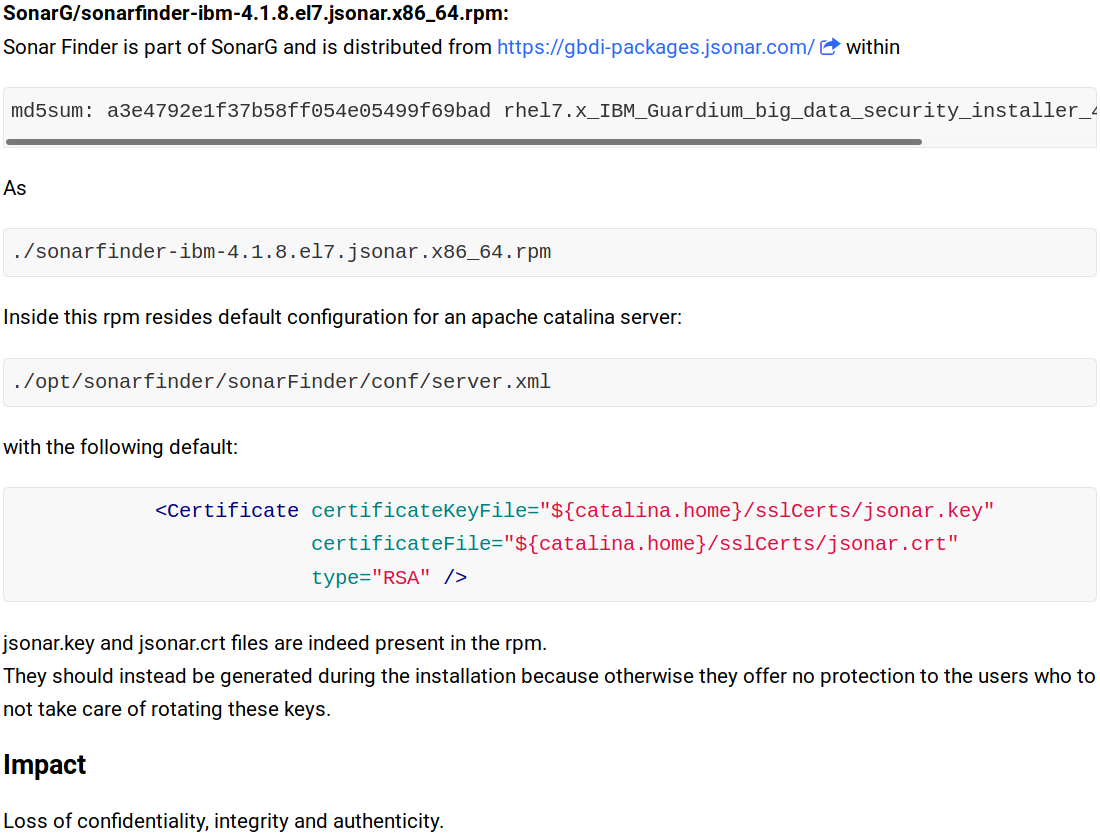
\includegraphics[width=250px]{./badpractice1.png}
            \end{figure}

            \begin{figure}[h!]
              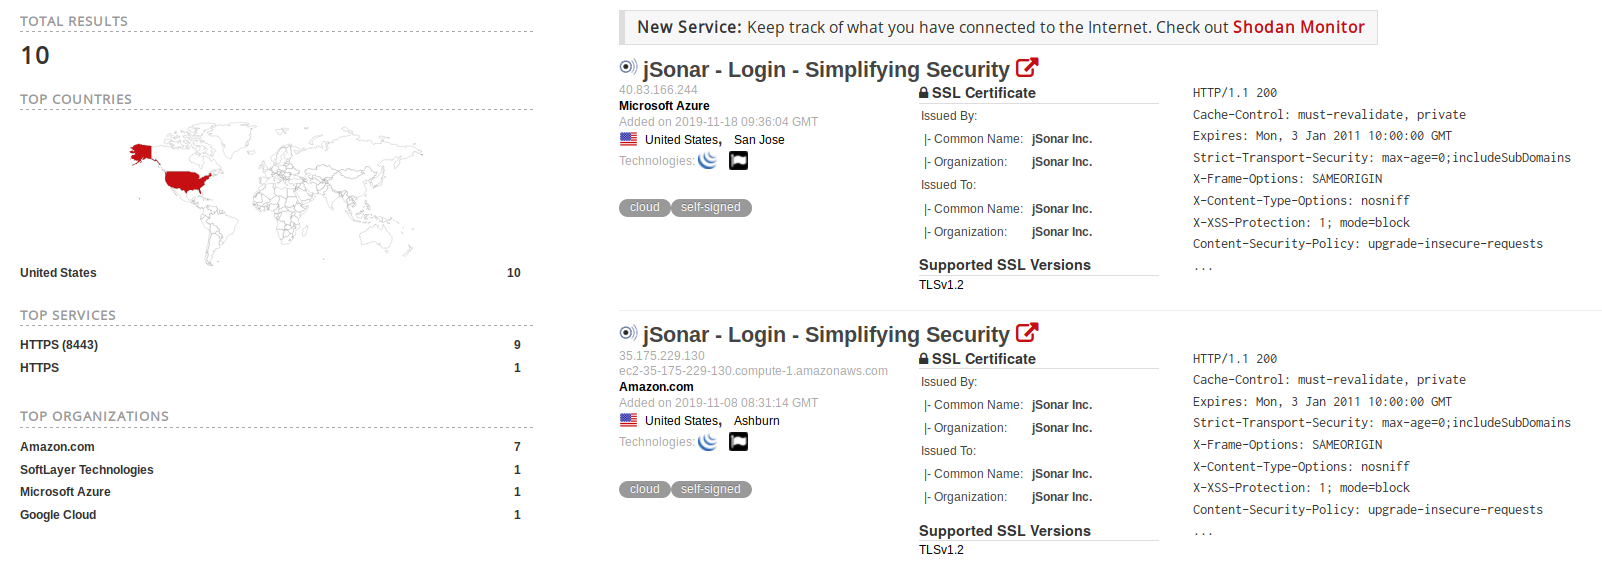
\includegraphics[width=250px]{./badpractice3.png}
            \end{figure}

            \begin{figure}[h!]
              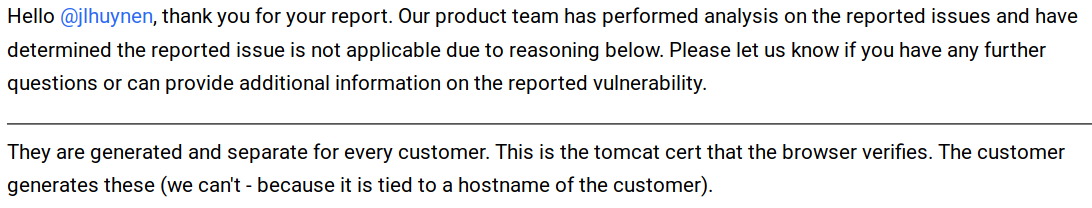
\includegraphics[width=250px]{./badpractice2.png}
            \end{figure}

\end{frame}

\begin{frame}
        \frametitle{XOR encryption}
            \begin{figure}[h!]
              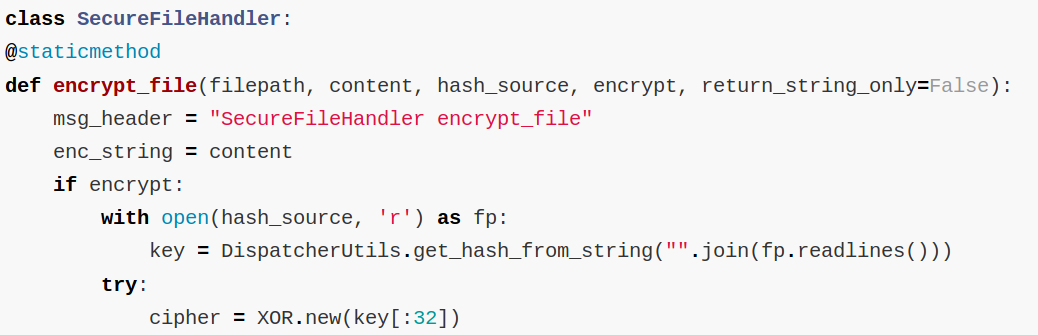
\includegraphics[width=250px]{./xorencryption.png}
            \end{figure}
\end{frame}

\begin{frame}[allowframebreaks]
        \frametitle{``Custom'' Key derivation function}
           \begin{figure}[h!]
              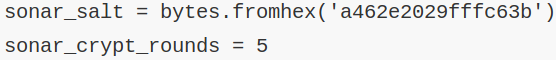
\includegraphics[width=250px]{./kdf1.png}
           \end{figure}
           \begin{figure}[h!]
              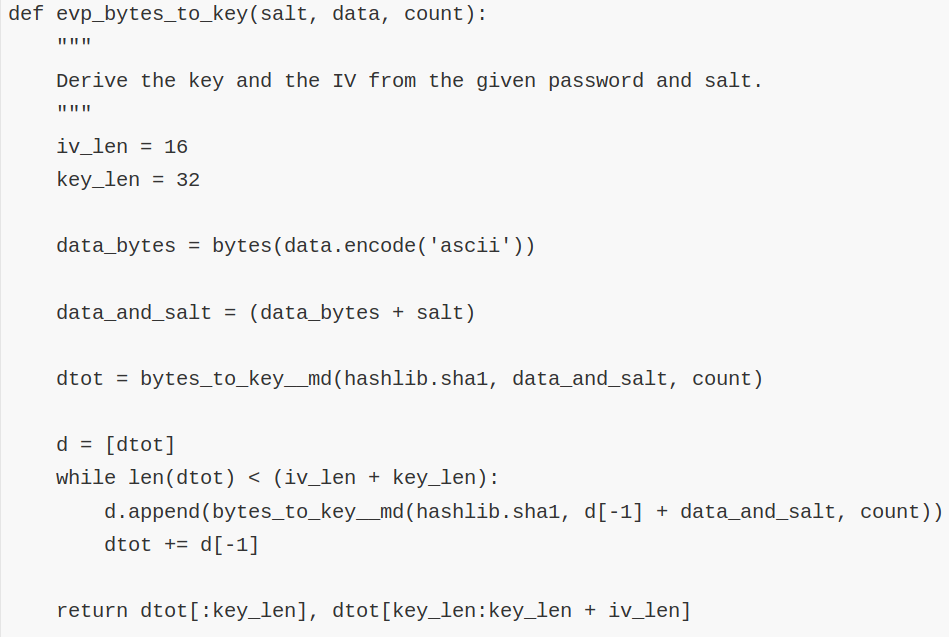
\includegraphics[width=250px]{./kdf2.png}
           \end{figure}
\end{frame}

\begin{frame}
        \frametitle{AES-ECB}
            \begin{figure}[h!]
              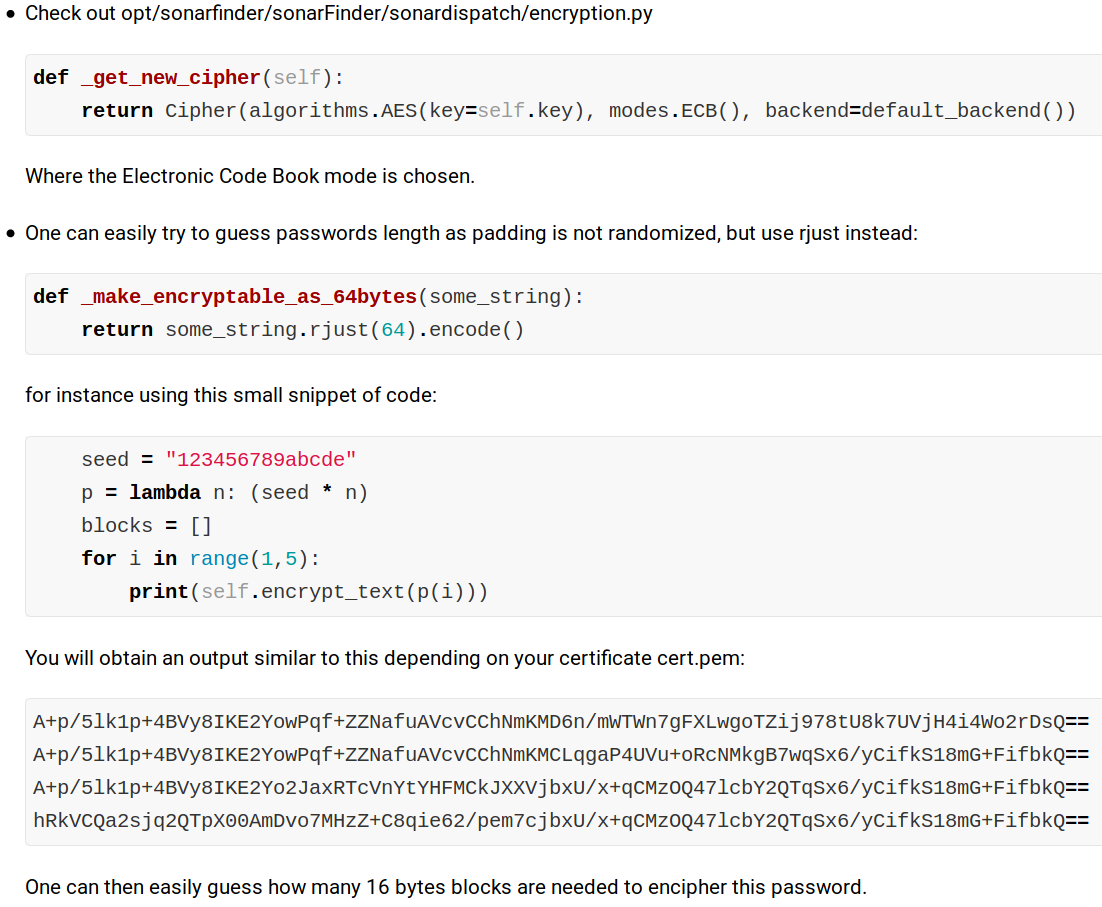
\includegraphics[width=250px]{./ecb.png}
            \end{figure}
\end{frame}


\begin{frame}
  \begin{center}
    {\bf Understanding RSA}
  \end{center}
\end{frame}

\begin{frame}
  \frametitle{RSA Basics}
  Ron {\bf R}ivest, Adi {\bf S}hamir, and Leonard {\bf A}dleman in 1977:
  \begin{itemize}
    \item asymmetric crypto system,
    \item can encrypt and sign,
    \item messages are big numbers,
    \item encryption is basically multiplication of big numbers,
    \item creates a \textit{trapdoor permutation}: turning x in y is easy, but
      finding x from y is hard.
  \end{itemize}

\end{frame}
\begin{frame}[fragile]
  \frametitle{RSA ``by hand''}
  \begin{itemize}
  \item {\bf Hands-on,} a sagemath script that is a toy example of RSA: 

\begin{lstlisting}
cd ~/hands-on/UsingRSA
sage rsa.sage
\end{lstlisting}
\item {\bf Outputs:}
\end{itemize}
\begin{lstlisting}[basicstyle=\tiny]
PlainText is: 1234567890
p = random_prime(2^32) = 2312340619
q = random_prime(2^32) = 2031410981
n = p*q = 4697314125248937239
phi = (p-1)*(q-1) = 4697314120905185640
e = random_prime(phi) = 2588085603940229747
d = xgcd(e,phi)[1] = -2102894211931680277
Does d*e == 1?
 mod(d*e, phi) = 1
CipherText y = power_mod(x, e, n) = 1454606910711062745
Decrypted CT is: 1234567890
\end{lstlisting}
\end{frame}

\begin{frame}[fragile]
  \frametitle{RSA - Use with openssl}
  \begin{itemize}
  \item {\bf Hands-on}:

\begin{lstlisting}
~/hands-on/UsingRSA
\end{lstlisting}

   \item Decrypt message.bin
   \item generate a new private key,
   \item generate the corresponding public key,
   \item use this new key to encrypt a message,
   \item use this new key to decrypt a message. 
   
  \end{itemize}
\end{frame}

\begin{frame}
  \frametitle{With only one key}
  Several potential weaknesses:
  \begin{itemize}
    \item Key size too small: keys up to 1024 bits are breakable given the
      right means,
    \item close p and q,
    \item unsafe primes, smooth primes,
    \item broken primes (FactorDB, Debian OpenSSL bug).
    \item signing with RSA-CRT (instead of RSA-PSS)
  \end{itemize}

\end{frame}

\begin{frame}
  \frametitle{With a set of  keys}
  Several potential weaknesses:
  \begin{itemize}
   \item share moduli: if n1 = n2 then the keys share p and q,
   \item share p or q,
  \end{itemize}
 \vspace{10mm}
  {\bf In both case, it is trivial to recover the private keys.}
\end{frame}


\begin{frame}[fragile]
  \frametitle{Breaking small keys\footnote{https://www.sjoerdlangkemper.nl/2019/06/19/attacking-rsa/}}
  \begin{itemize}
\item {\bf Hands-on}:

\begin{lstlisting}
~/hands-on/SmallKey
\end{lstlisting}

   \item what is the key size of smallkey?
   \item what is n?
   \item what is the public exponent?
   \item what is n in base10?
   \item what are p and q?
   
  \end{itemize}

  \vspace{8mm}
  {\bf Let's generate the private key: }using p, then using q.
  
\end{frame}

\begin{frame}[fragile]
  \frametitle{Close Prime Factors}
  \begin{itemize}
\item {\bf Hands-on}:

\begin{lstlisting}
~/hands-on/ClosePQ
\end{lstlisting}

   \item use Fermat Algorithm\footnote{\url{http://facthacks.cr.yp.to/fermat.html}} to find {\bf both p and q:}

\begin{lstlisting}[basicstyle=\tiny]
def fermatfactor(N):
  if N <= 0: return [N]
  if is_even(N): return [2,N/2]
  a = ceil(sqrt(N))
  while not is_square(a^2-N):
    a = a + 1
  b = sqrt(a^2-N)
  return [a - b,a + b]
\end{lstlisting}

  \end{itemize}
 
\end{frame}

\begin{frame}[fragile]
  \frametitle{Shared prime factors}
     Researchers have shown that several devices generated their keypairs
   at boot time without enough entropy\footnote{Bernstein, Heninger, and Lange: \url{http://facthacks.cr.yp.to/}}:
   
\begin{lstlisting}[language=python, basicstyle=\tiny]
prng.seed(seed)
p = prng.generate_random_prime()
// prng.add_entropy()
q = prng.generate_random_prime()
n = p*q
\end{lstlisting}

Given n=pq and n' = pq' it is trivial to recover the shared p by computing their
{\bf Greatest Common Divisor (GCD)}, and therefore {\bf both private
  keys}\footnote{\url{http://www.loyalty.org/~schoen/rsa/}}.\\
\vspace{5mm}
``They cracked about 13000 of them''
\end{frame}

\begin{frame}[fragile]
  \frametitle{Shared prime factors}
  \begin{itemize}
\item {\bf Hands-on}:

\begin{lstlisting}
~/hands-on/SharedPrimeFactor
\end{lstlisting}

\item Read README.txt, you have a challenge to solve :

  \begin{itemize}
  \item the \emph{answers} folder should be left alone for now,
  \item \emph{scripts} contains scripts that may be useful
    to solve the challenge,
  \item \emph{attempts} may hold your attempt are
    generating private keys. 
  \item \emph{bgcd-bd.sage} contains Daniel J. Berstein's algorithm for computing RSA
    collisions in batches.
  \end{itemize}

  \end{itemize}
 
\end{frame}


\begin{frame}
  \begin{center}
    {\bf Hands-on: Exploiting Weaknesses in RSA}\\
    {\bf -- at bigger scale --}\\
  \end{center}
\end{frame}

\begin{frame}
  \frametitle{Snake Oil Crypto\footnote{\url{https://github.com/d4-project/snake-oil-crypto}} - Problem Statement}
  We reckon that IoT devices {\bf are often the weakest devices} on a network:

        \begin{itemize}
        \item Usually the result of cheap engineering,
        \item sloppy patching cycles,
        \item sometimes forgotten--not monitored (remember the printer sending sysmon?),
        \item few hardening features enabled.
        \end{itemize}

        \vspace{10 mm} 

{\bf We feel a bit safer when they use TLS, but we what you now know about RSA, should we?}
\end{frame}

\begin{frame}
   \frametitle{Snake Oil Crypto - GCD}
   In Snake-Oil-Crypto we compute GCD\footnote{using Bernstein's Batch GCD algorithm} between:
   
   \begin{itemize}
     \item between certificates having the same issuer,
     \item between certificates having the same subject,
     \item on keys collected from various sources (PassiveSSL, Certificate Transparency,
       shodan, censys, etc.),
     \item python + redis + postgresql~\footnote{\url{https://github.com/D4-project/snake-oil-crypto/}}
   \end{itemize}

\vspace{10 mm}
  {\bf ``Check all the keys that we know of for vendor X''}

\end{frame}

\begin{frame}
   \frametitle{Snake Oil Crypto - GCD}

   Quick Demo:
   \begin{itemize}
   \item Let's check how strong are the RSA keys in our database...
   \item check some results on https://misp-eurolea.enforce.lan
   \item how bad can it be?
   \item do you find some vendors we should notify?
   \end{itemize}

\end{frame}

\begin{frame}
   \frametitle{Snake Oil Crypto - MISP feed}
\begin{figure}
\centering
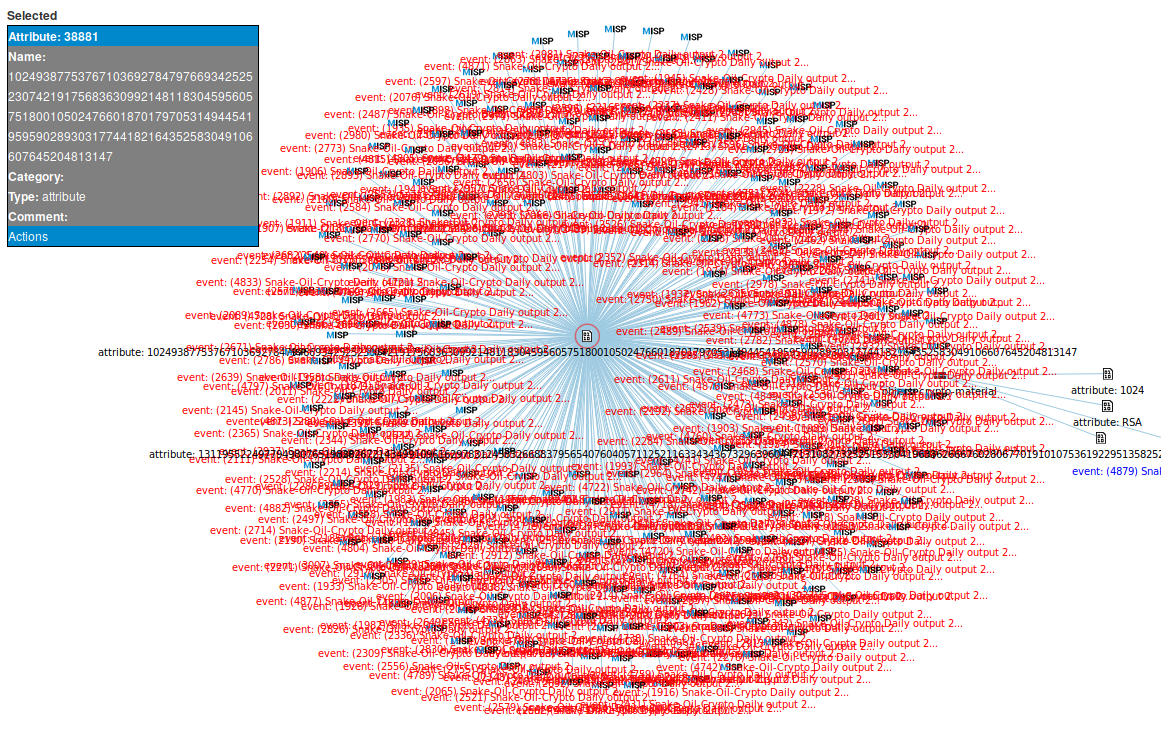
\includegraphics[width=\textwidth]{misp.png}
\end{figure}
\end{frame}

\begin{frame}
   \frametitle{Snake Oil Crypto - MISP feed}
   The MISP feed:
   \begin{itemize}
     \item {\bf Allows} for checking automatic checking by an IDS on hashed values,
     \item {\bf contains} thousands on broken keys from a dozen of vendors,
     \item {\bf will be accessible upon request (info@circl.lu).}
   \end{itemize}

   In the future:
    \begin{itemize}
     \item {\bf Automatic} the vendor checks by performing TF-IDF on x509's subjects, 
     \item {\bf automatic} vendors notification.
    \end{itemize}

\end{frame}


\begin{frame}
  \begin{center}
    {\bf Hands-on: Exploiting Weaknesses in RSA}\\
    {\bf -- enter D4-project --}\\
  \end{center}
\end{frame}

\begin{frame}
        \frametitle{Problem statement}
        \begin{itemize}
                \item CSIRTs (or private organisations) build their {\bf own honeypot, honeynet or blackhole monitoring network}
                \item Designing, managing and operating such infrastructure is a tedious and resource intensive task
                \item {\bf Automatic sharing} between monitoring networks from different organisations is missing
                \item Sensors and processing are often seen as blackbox or difficult to audit

        \end{itemize}
\end{frame}

\begin{frame}
 \frametitle{Objective}
 \begin{itemize}
         \item Based on our experience with
           MISP\footnote{\url{https://github.com/MISP/MISP}} where sharing
           played an important role, we transpose the model in D4 project
         \item Keeping the protocol and code base {\bf simple and minimal}
         \item Allowing every organisation to {\bf control and audit their own sensor network}
         \item Extending D4 or {\bf encapsulating legacy monitoring protocols} must be as simple as possible
         \item Ensuring that the sensor server has {\bf no control on the sensor} (unidirectional streaming)
         \item Don't force users to use dedicated sensors and allow {\bf flexibility of sensor support} (software, hardware, virtual)

 \end{itemize}
\end{frame}

\begin{frame}
\frametitle{D4 Overview}
        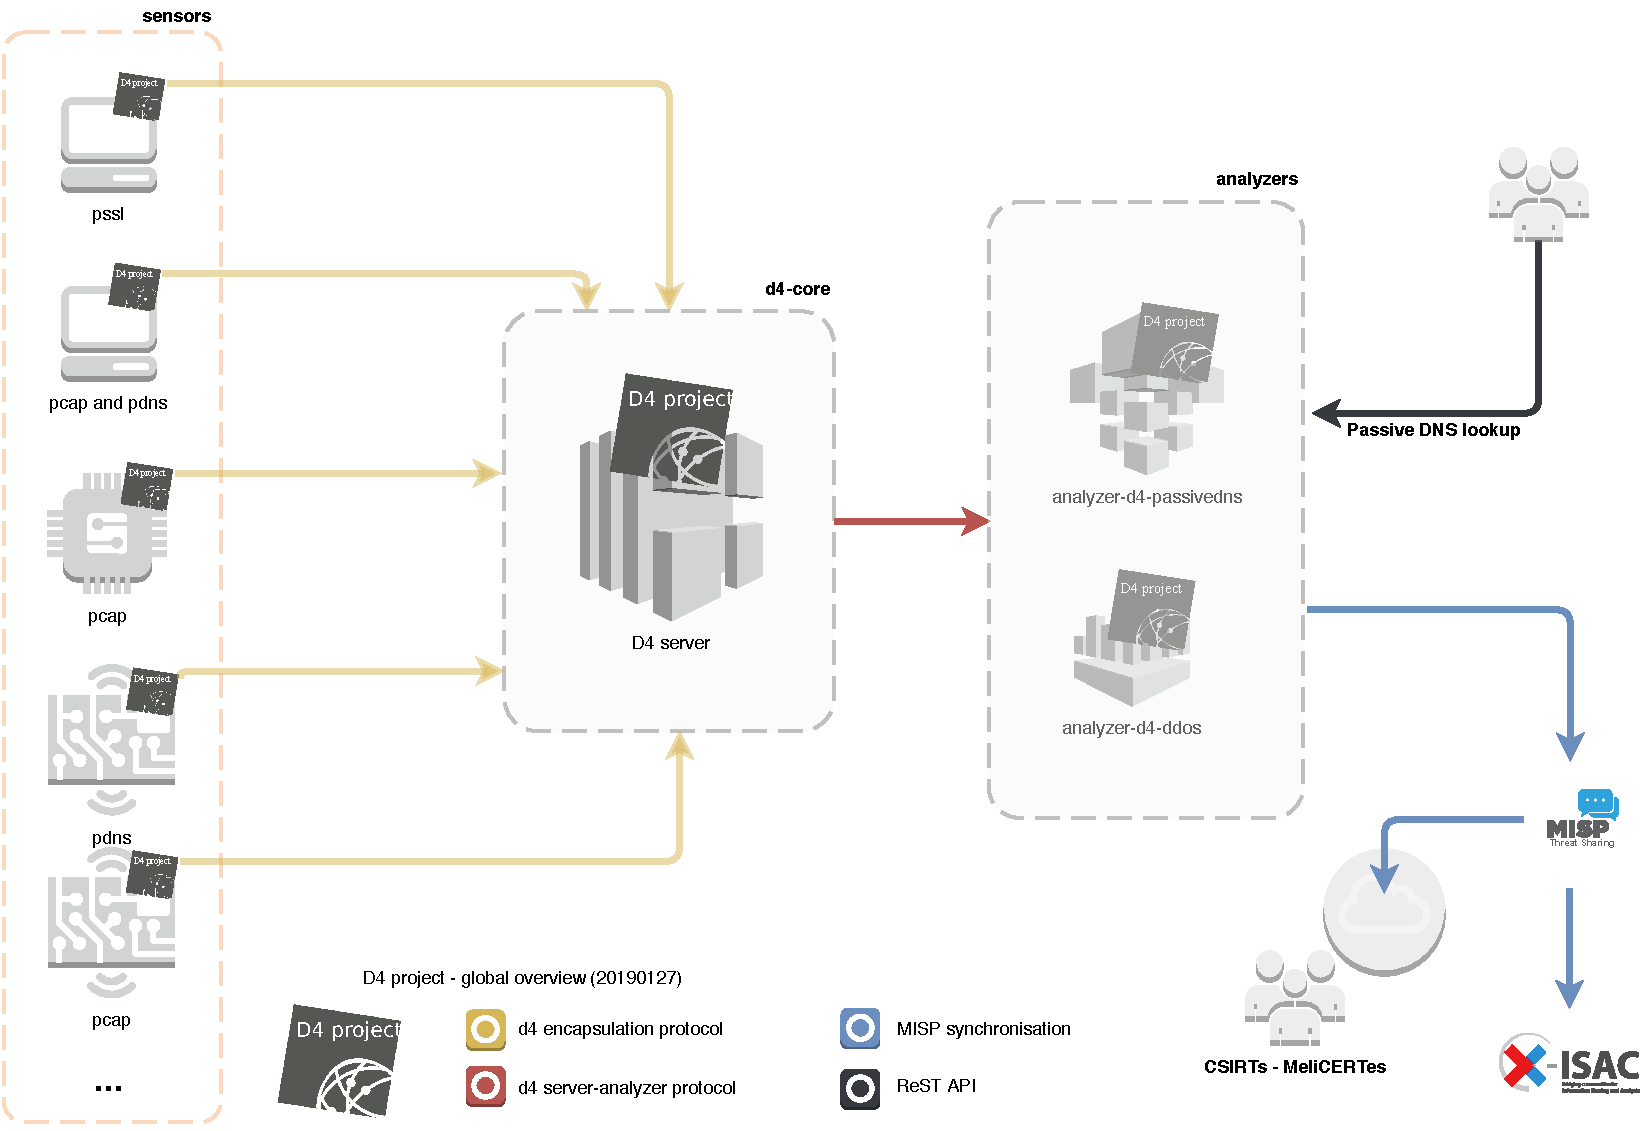
\includegraphics[scale=0.38]{d4-overview.pdf}
\end{frame}


\begin{frame}
\frametitle{D4 Overview - Connecting Sensor Networks}
        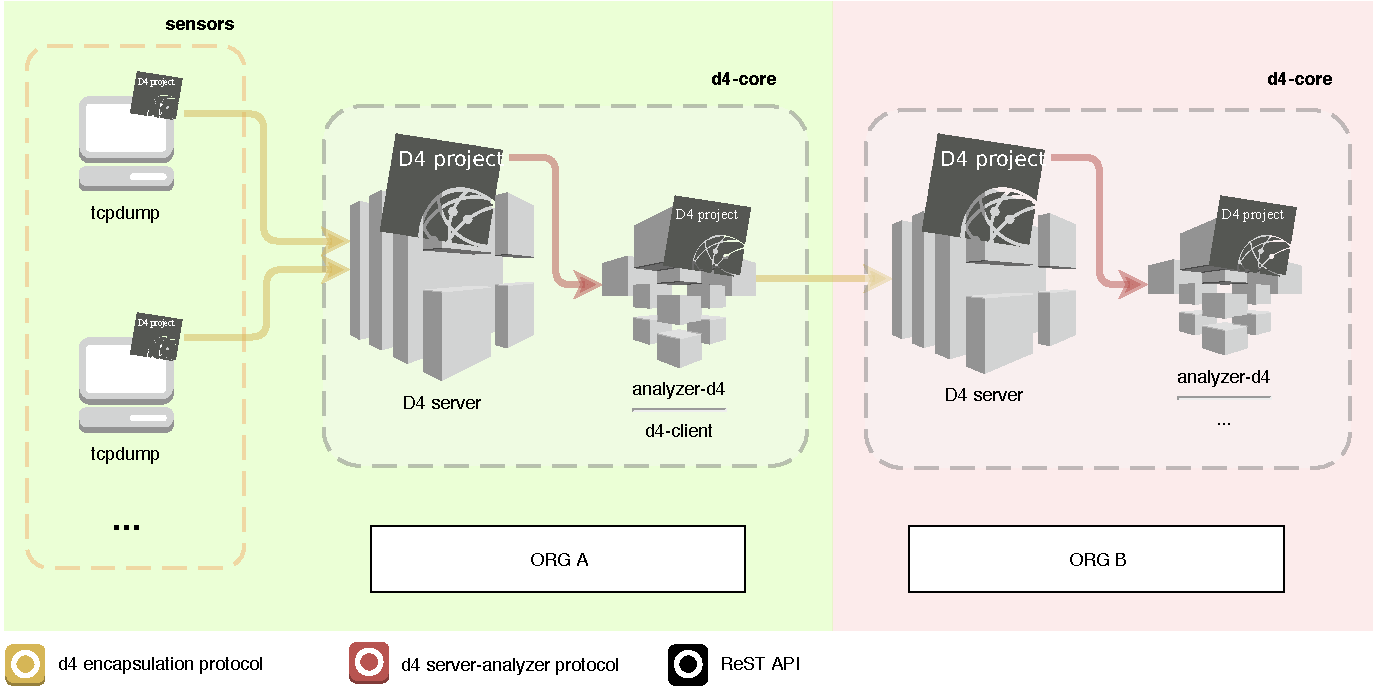
\includegraphics[scale=0.46]{mixing-d4-1.pdf}
\end{frame}


\begin{frame}
  \frametitle{D4 - TLS Fingerprinting}
        {\bf Keep} a log of links between:
        \begin{itemize}
          \item x509 certificates,
          \item ports,
          \item IP address,
          \item client (ja3),
          \item server (ja3s),
        \end{itemize}
        \begin{quote}
        ``JA3 is a method for creating SSL/TLS client fingerprints that should be easy to produce on any platform and can be easily shared for threat intelligence.''\footnote{https://github.com/salesforce/ja3}
        \end{quote}

         {\bf Pivot} on additional data points during Incident Response 
\end{frame}


\begin{frame}[fragile]
  \frametitle{D4 - TLS Fingerprinting}

\begin{itemize}

   \item {\bf Hands-on}:

\begin{lstlisting}
~/hands-on/TLSinspection
\end{lstlisting}

   \item open stripped.pcap
   \item what is the admin password?
   \item bummer, it's encrypted,
   \item what is the admin password?
   
  \end{itemize}

  \vspace{8mm}
  {\bf D4 - full chain demo.}
 
\end{frame}


\begin{frame}
  \frametitle{First release}
  \begin{itemize}
  \item[\checkmark] sensor-d4-tls-fingerprinting
    \footnote{\url{github.com/D4-project/sensor-d4-tls-fingerprinting}}:
    {\bf Extracts} and {\bf fingerprints} certificates, and {\bf computes} TLSH fuzzy hash.
  \item[\checkmark] analyzer-d4-passivessl
    \footnote{\url{github.com/D4-project/analyzer-d4-passivessl}}:
    {\bf Stores} Certificates / PK details in a PostgreSQL DB.
  \item snake-oil-crypto 
    \footnote{\url{github.com/D4-project/snake-oil-crypto}}:
    {\bf Performs} crypto checks, push results in MISP for notification
  \item lookup-d4-passivessl
    \footnote{\url{github.com/D4-project/lookup-d4-passivessl}}:
    {\bf Exposes} the DB through a public REST API.
  \end{itemize} 
\end{frame}

\begin{frame}
\frametitle{Get in touch if you want to join/support the project, host a passive ssl sensor or contribute}
\begin{itemize}
\item Collaboration can include research partnership, sharing of collected streams or improving the software.
\item Contact: info@circl.lu
\item \url{https://github.com/D4-Project} -  \url{https://twitter.com/d4_project}
\end{itemize}
\end{frame}

\nocite{*} 
\begin{frame}[allowframebreaks]
        \frametitle{References}
        \bibliographystyle{amsalpha}
        \bibliography{references.bib}
\end{frame}

\end{document}
